\section{Escenario B: ampliar buffer o contratar un cuarto analista}

\subsection{Comparación bajo demanda base}

La Tabla~\ref{tab:escenario-b-base} compara las dos alternativas con la demanda
base. Ambas reducen la pérdida de alertas en más del $94$\,\%: $K=16$ deja
$\loss=0{,}019$\,\% y $s=4$ deja $0{,}021$\,\%. La diferencia entre ambas es
estadísticamente indistinguible: su intervalo de confianza del 95\,\% contiene
el cero. Sin embargo, los tiempos de espera separan claramente las opciones.
Con $K=16$ las esperas incluso aumentan respecto del caso base
($\Wqone=2{,}344$ y $\Wqtwo=7{,}183$ min), porque el buffer más grande permite
acumular más alertas. Con $s=4$ las esperas caen a
$\Wqone=0{,}659$ y $\Wqtwo=1{,}282$ min.

\begin{table}[H]
\centering
\small
% Tabla generada automáticamente por simulacion_colas.report.
% No editar a mano: regenerar con `python -m simulacion_colas report`.
\begin{tabular}{lrrr}
\toprule
Métrica & Base & $K=16$ & $s=4$ \\
\midrule
$P_{\text{loss}}$ (\%) & 0,385 $\pm$ 0,048 & 0,019 $\pm$ 0,012 & 0,021 $\pm$ 0,011 \\
Utilización (\%) & 68,87 $\pm$ 0,33 & 69,14 $\pm$ 0,33 & 51,85 $\pm$ 0,25 \\
$W_{q1}$ (min) & 2,267 $\pm$ 0,049 & 2,344 $\pm$ 0,054 & 0,659 $\pm$ 0,025 \\
$W_{q2}$ (min) & 6,417 $\pm$ 0,180 & 7,183 $\pm$ 0,259 & 1,282 $\pm$ 0,050 \\
$W_1$ (min) & 22,260 $\pm$ 0,060 & 22,339 $\pm$ 0,065 & 20,654 $\pm$ 0,042 \\
$W_2$ (min) & 17,250 $\pm$ 0,187 & 18,018 $\pm$ 0,261 & 12,117 $\pm$ 0,070 \\
$L_q$ (trabajos) & 0,750 $\pm$ 0,022 & 0,834 $\pm$ 0,030 & 0,161 $\pm$ 0,006 \\
\bottomrule
\end{tabular}

\caption{Escenario B bajo demanda base: media $\pm$ semiancho del IC95\,\%.}
\label{tab:escenario-b-base}
\end{table}

\subsection{Sensibilidad bajo la sobrecarga del Escenario A}

La Tabla~\ref{tab:escenario-b-sobrecarga} repite la comparación con
$\lambda_2=0{,}14$. Aquí la diferencia en pérdida sí es clara: $K=16$ deja
$\loss=0{,}395$\,\%, mientras que $s=4$ la reduce a $0{,}129$\,\%. La
diferencia pareada es $-0{,}266$ puntos porcentuales, con IC95\,\%
$[-0{,}339;-0{,}193]$. Además, $s=4$ mantiene la espera preventiva en
$2{,}519$ minutos frente a $17{,}414$ minutos con $K=16$.

\begin{table}[H]
\centering
\small
% Tabla generada automáticamente por simulacion_colas.report.
% No editar a mano: regenerar con `python -m simulacion_colas report`.
\begin{tabular}{lrrr}
\toprule
Métrica & Base A & $K=16$ & $s=4$ \\
\midrule
$P_{\text{loss}}$ (\%) & 2,220 $\pm$ 0,152 & 0,395 $\pm$ 0,082 & 0,129 $\pm$ 0,029 \\
Utilización (\%) & 81,65 $\pm$ 0,33 & 83,19 $\pm$ 0,38 & 62,56 $\pm$ 0,30 \\
$W_{q1}$ (min) & 3,074 $\pm$ 0,058 & 3,311 $\pm$ 0,061 & 1,065 $\pm$ 0,022 \\
$W_{q2}$ (min) & 11,663 $\pm$ 0,260 & 17,414 $\pm$ 0,703 & 2,519 $\pm$ 0,076 \\
$W_1$ (min) & 23,065 $\pm$ 0,071 & 23,305 $\pm$ 0,070 & 21,060 $\pm$ 0,037 \\
$W_2$ (min) & 22,495 $\pm$ 0,276 & 28,245 $\pm$ 0,719 & 13,350 $\pm$ 0,101 \\
$L_q$ (trabajos) & 1,741 $\pm$ 0,040 & 2,585 $\pm$ 0,103 & 0,404 $\pm$ 0,012 \\
\bottomrule
\end{tabular}

\caption{Escenario B bajo la sobrecarga del Escenario A: media $\pm$ semiancho del IC95\,\%.}
\label{tab:escenario-b-sobrecarga}
\end{table}

\begin{figure}[H]
\centering
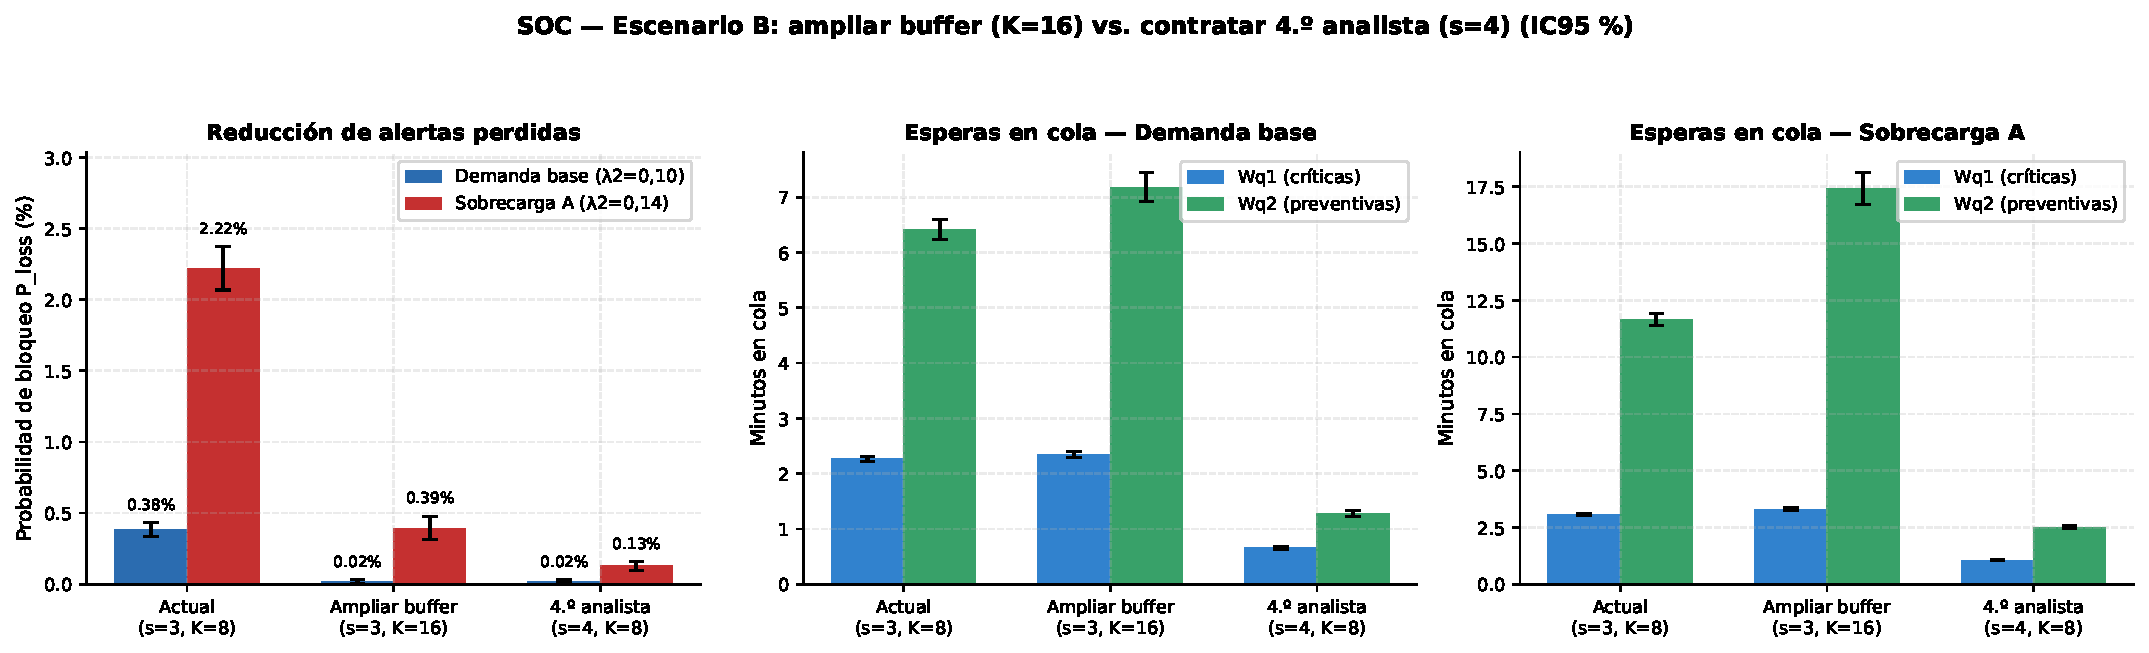
\includegraphics[width=\linewidth]{soc_scenario_b.pdf}
\caption{Escenario B: pérdida de alertas y esperas bajo demanda base y bajo sobrecarga.}
\label{fig:escenario-b}
\end{figure}

\subsection{Recomendación}

\textbf{¿Cuál alternativa reduce más drásticamente las alertas perdidas?} Bajo
la demanda base, ambas son equivalentes en pérdida. Bajo la sobrecarga
previsible del Escenario A, el cuarto analista es claramente superior
($0{,}129$\,\% frente a $0{,}395$\,\%). \textbf{¿Cuál optimiza mejor los
tiempos de espera?} El cuarto analista, en ambos regímenes: reduce la espera
crítica un $71{,}9$\,\% y la preventiva un $82{,}2$\,\% bajo demanda base;
bajo sobrecarga, reduce la espera preventiva de $17{,}414$ a $2{,}519$ minutos.

La razón es estructural: ampliar el buffer no añade capacidad de servicio,
solo permite que las alertas esperen más tiempo antes de bloquearse. Cuando el
sistema se congestiona, el buffer se llena y la pérdida reaparece, mientras que
los tiempos de espera crecen. Un analista adicional aumenta la capacidad de
servicio, reduce la utilización por analista y disminuye simultáneamente
pérdidas y esperas. Por ello, \textbf{se recomienda contratar el cuarto
analista manteniendo $K=8$} ($s=4$, $K=8$).
